\documentclass[tesi]{subfiles}

\IfEq{\jobname}{\detokenize{tesi}}{}{%
    \externaldocument{Chapter4}
}
\begin{document}

\chapter{System Development}
\label{ch:System Development}
This chapter analyses how the system has been developed, mainly focusing on:

\begin{itemize}
\item How data are collect.
\item Processing which they are subject to, and how the indexes are determined.
\item Data storing.
\item Viewing on interactive map.
\end{itemize}

\noindent The figure below shows the structure of the system.


\begin{figure}[H]
\centering
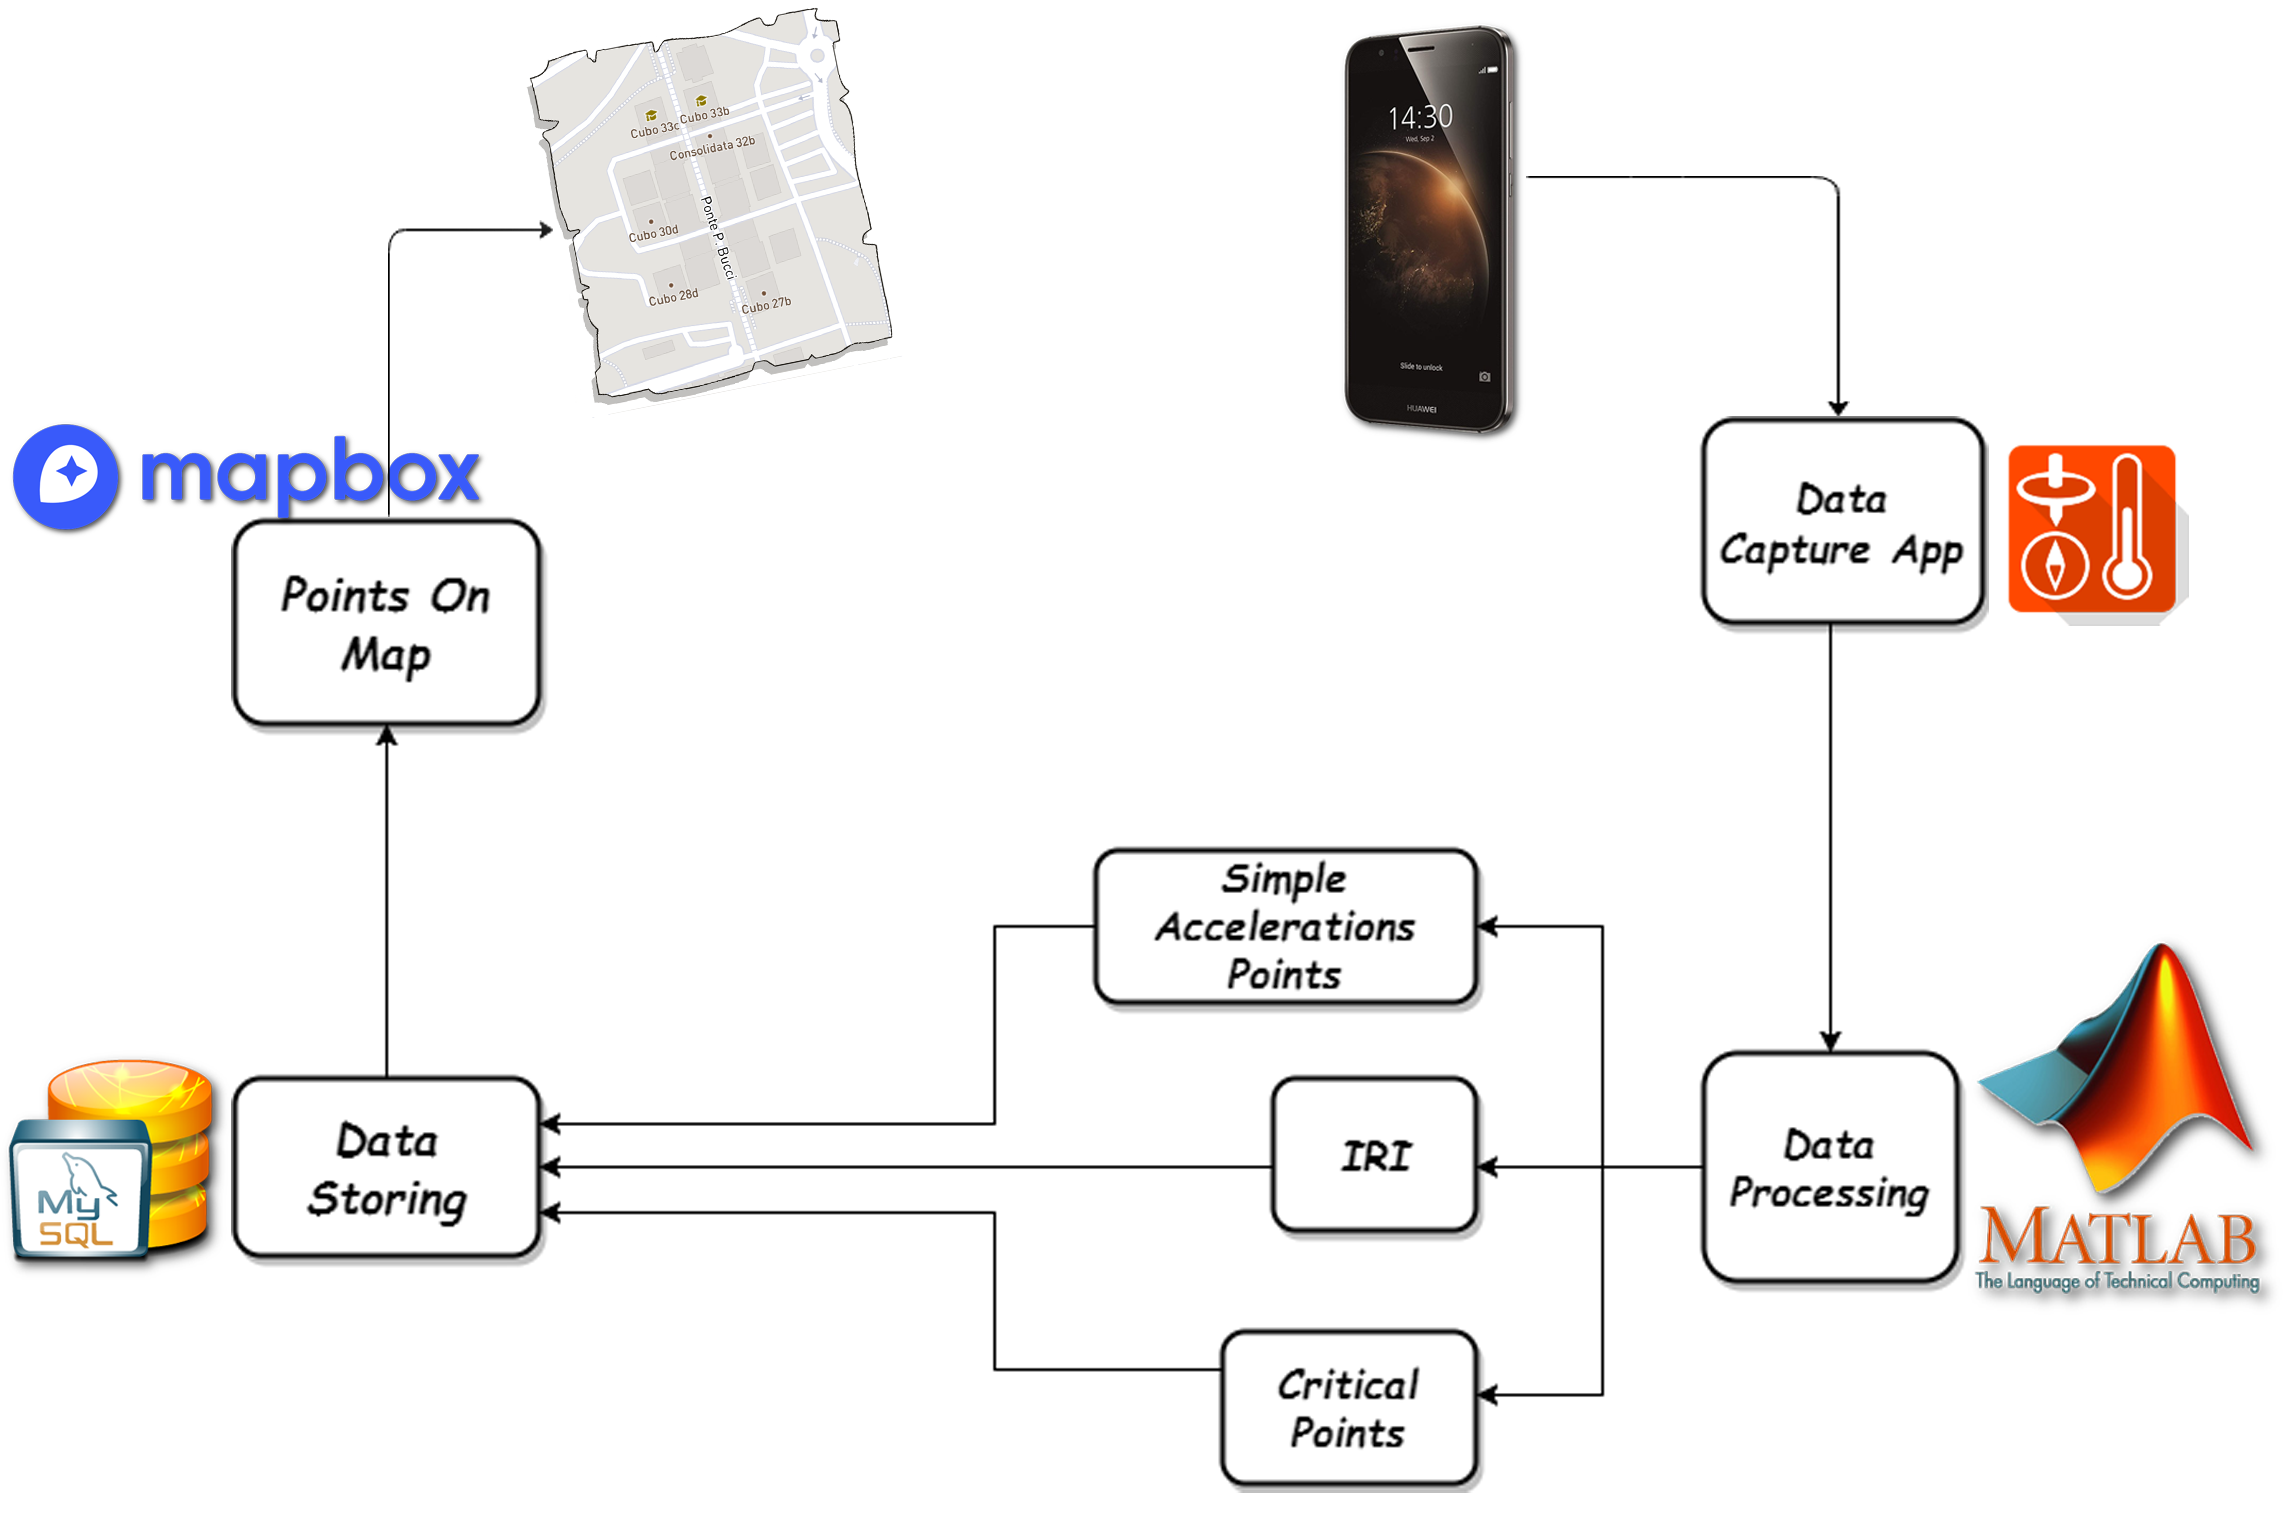
\includegraphics[scale=0.6]{WorkFlow}
\caption{System Structure}

\end{figure}\label{fig:System Structure}

\section{Data Collect}\label{sc:Data Collect}
Initially, the smartphone was fixed up at the windshield of the car by an arm support, forming a $90°$ angle between the phone and the vehicle axes.\\
However, during travel, the support was subject to vibrations that caused additional noise in the data, and could also be subject to movements due to the nature of the support itself and the road surface conditions, thus changing the integrity of the data.\\
The smartphone was then mounted horizontally on the car dashboard, forming a proximal $0°$ angle with the same, using a non-slip mat, where the perceived vibrations are proportional at the vibrations sensed by the car, the movements of the smartphones are almost null.\\
The AndroSensors application available on the PlayStore was used to make the measurements. That allows us to perform contemporary measurements of various sensors.\\
For our purpose were monitoring:

\begin{itemize}
\item Accelerometer.
\item Linear Accelerometer.
\item GPS.
\item Orientation.
\item Date
\item Time
\end{itemize}


\noindent The data are updated at the highest frequency \textit{"Very Fast"}, while the sampling frequency can be chosen within a range that goes:


\begin{center}
$fs_{min} \quad <= \thinspace f_{s} \thinspace <= \thinspace fs_{max}$\\
$200 \thinspace Hz \quad <= \thinspace f_{s} \thinspace <= \thinspace 1 \thinspace Hz$\\
$0,005 \thinspace s <= \thinspace f_{s} \thinspace <= \thinspace 1 \thinspace s $
\end{center}


\noindent Choosing a very low sampling frequency (for example, $fs_{min}$, sensor values may be inconsistent at writing time due to their fast sampling frequency, however, the higher is the sample rate, higher is the accuracy and quality of the information.\\
Conversely, choosing a very high sampling frequency, (for example, $fs_{max}$), we will have very disconnected data, in fact, if you are supposed to travel at a speed of $130 \thinspace \si{\km\per\hour}$, you will have a data every $36,11  \si{\meter}$ of road, which is not favorable to the monitoring of road surface conditions.\\
Because of these reasons, was chosen a sampling frequency of:
\begin{center}
$fs = 100 \thinspace Hz; \quad fs = 0,01s; \quad fs = 10ms$
\end{center}

\noindent Which is stable, and for every second of recording we own $100$ sample of data for the previously listened sensors. The GPS still have the same number of data, but changing every second as the GPS sensor updates at a frequency of $1 \thinspace Hz$ (in some cases this frequency may be lower by reaching a maximum of $20 \thinspace Hz$).\\
Once the GPS signal has been established, it is possible to start recording the data.
 
 
 
 \section{Data Processing}\label{sc:Data Processing}
 Regarding data processing, 3 indexes will be extrapolated:
 
 \begin{itemize}
 \item Simple Accelerations Points
 \item Critical Points
 \item IRI
 \end{itemize}


\noindent Once the measurements are complete, the data will be saved inside a $.xls$ file

\noindent These will be processed with MATLAB (Matrix Laboratory) a multi-paradigm numerical computing environment, which makes numerical computing more easier and computationally faster than other programming paradigms.

\noindent Initially, the $.xls$ file will be read, and each column of it depending on the data nature (numeric or string) will be stored in a vector, which can be found in the MATLAB workspace.

\noindent Once the raw data has been read, it is possible starting calculating the indices.


\subsection{Simple Acceleration Points}\label{ssc:Simple Accelerations Points}
This index helps principally to show how the acceleration component changes depending on different points on the road surface.\\It notes that an appropriate methodology is needed to calculate the surface conditions because the representation of the acceleration signal alone would not be satisfactory to provide all the conditions of a given road segment.\\
This index will be calculated on a segment of a predetermined length ($distance_{segment}$) in which an $\chi$ value will be associated and calculated as follows:

\begin{center}
 $\chi \thinspace = \left( \sum \limits_{i=1}^{N} \thinspace a_{i} \right) \thinspace \dfrac{1}{N}$
\end{center}\label{eq:sap}


\noindent Where: $N$, is the number of GPS points necessary to reach a lenght of $distance_{segment}$, and $a_{i}$ is the processed acceleration value associated to $i$.


\noindent For example, if considering an urban road of more or less good conditions, the travel speed on it can not be elevated, so for each segment considered, we will have many values associated with it to handle during the processing, belong to several seconds of registration.\\
\noindent This means that at the time of the final calculation of the value, it will be averaged with many points. The end result will definitely have a small value. This value would indicate that the condition of the road surface it is almost perfect, although it is not really so, since considering urban roads, they may have various abnormalities.\\\\
\noindent Conversely, if taking into consideration a highway, the travel speed will be much higher so for each segment taken into considerations, the values to be handled are lower respect to a urban road. The final result will have a higher value, which suggests that road surface conditions are not good, although the surface of a highway is very comfortable and almost flat.\\\\
\noindent This value will be calculated by performing a few processing operations on it.\\\\


\noindent Considering the following signal:
\begin{figure}[H]
\centering
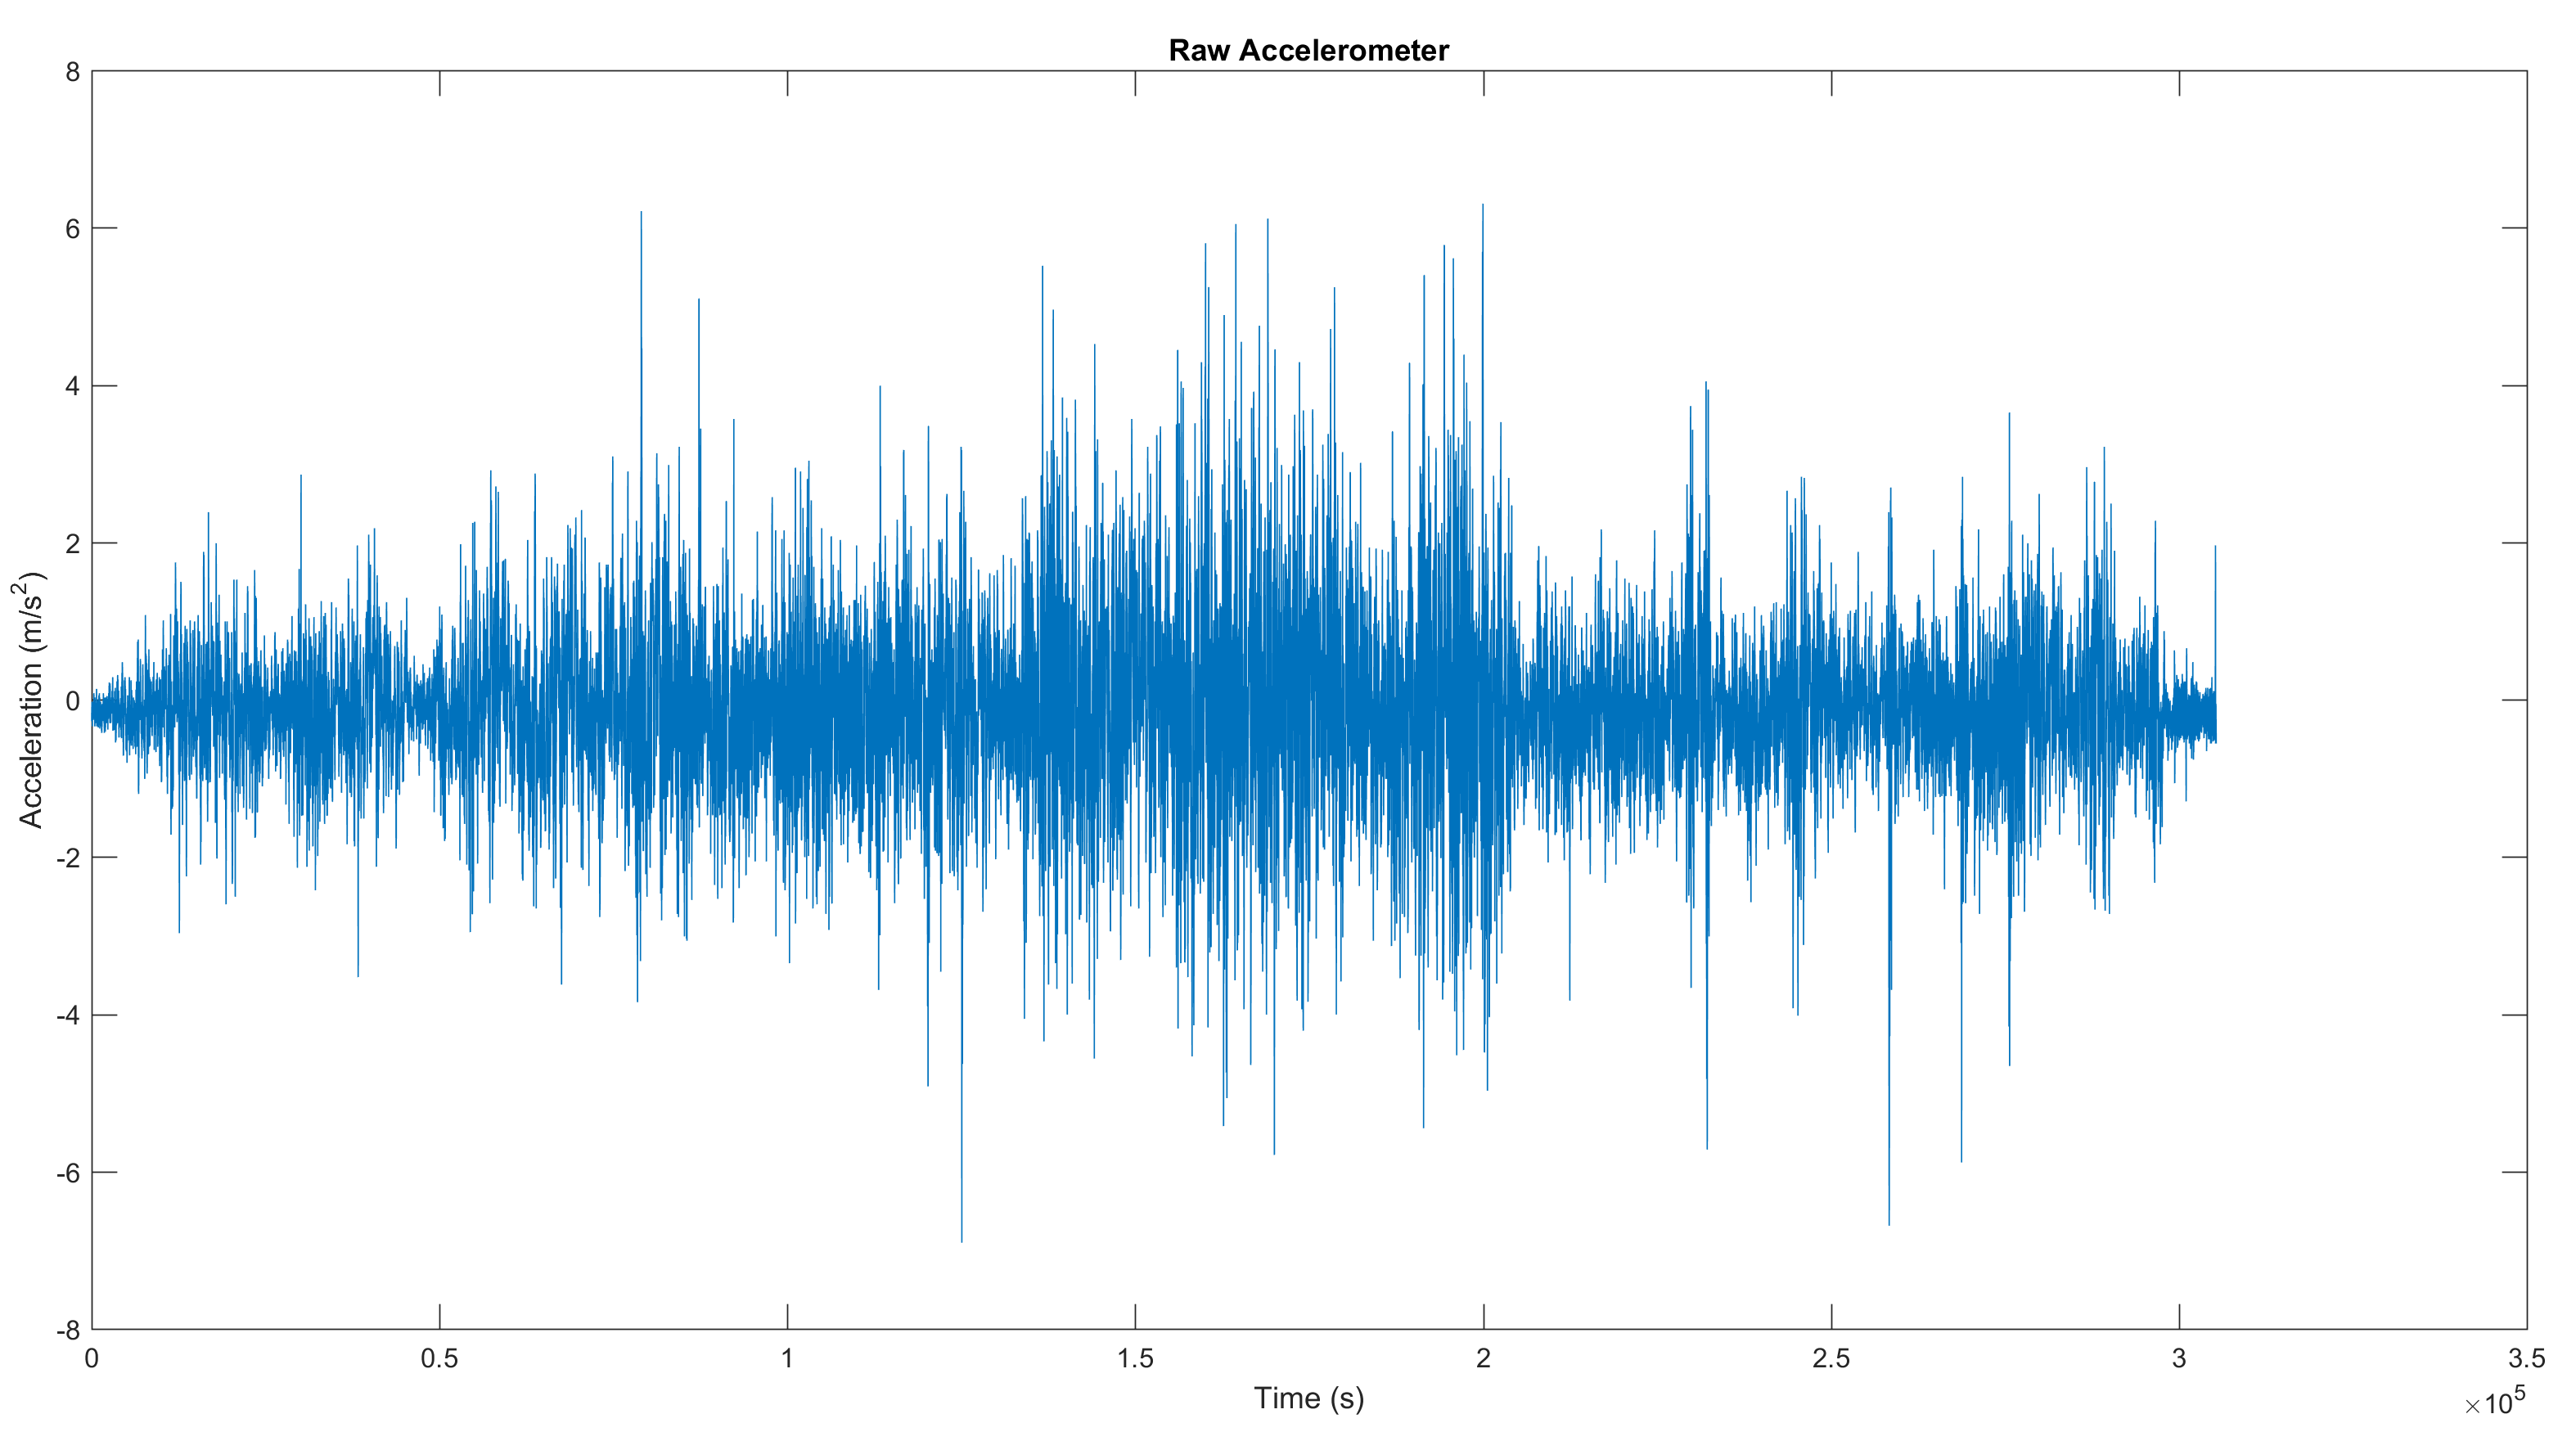
\includegraphics[scale=0.1]{SPARaw}
\end{figure}

\noindent The steps are as follows:

\begin{description}
\item[1. Accelerometer Reorentation:] First of all it is applied the procedure of Accelerometer reorientation explained in Chapter\ref{ch:Data Analysis} (section:\ref{sc:Accelerometer Reorientation}, on page: \pageref{sc:Accelerometer Reorientation}).
\item[2. GPS points division:] Next, the GPS points are subdivided according to the methodology explained in Chapter\ref{ch:Data Analysis} (section:\ref{sc:GPS points division}, on page: \pageref{sc:GPS points division}).
\item[3. Zero Velocity Filter:] This filter is the first operation that is performed on the data, applying it as explained in the Chapter\ref{ch:Data Analysis} (section:\ref{sc:Data Filtering}, on page:\pageref{sssc:Zero Velocity Filter}). A figure below show how the filter is applied on the Signal
\begin{figure}[H]
\centering
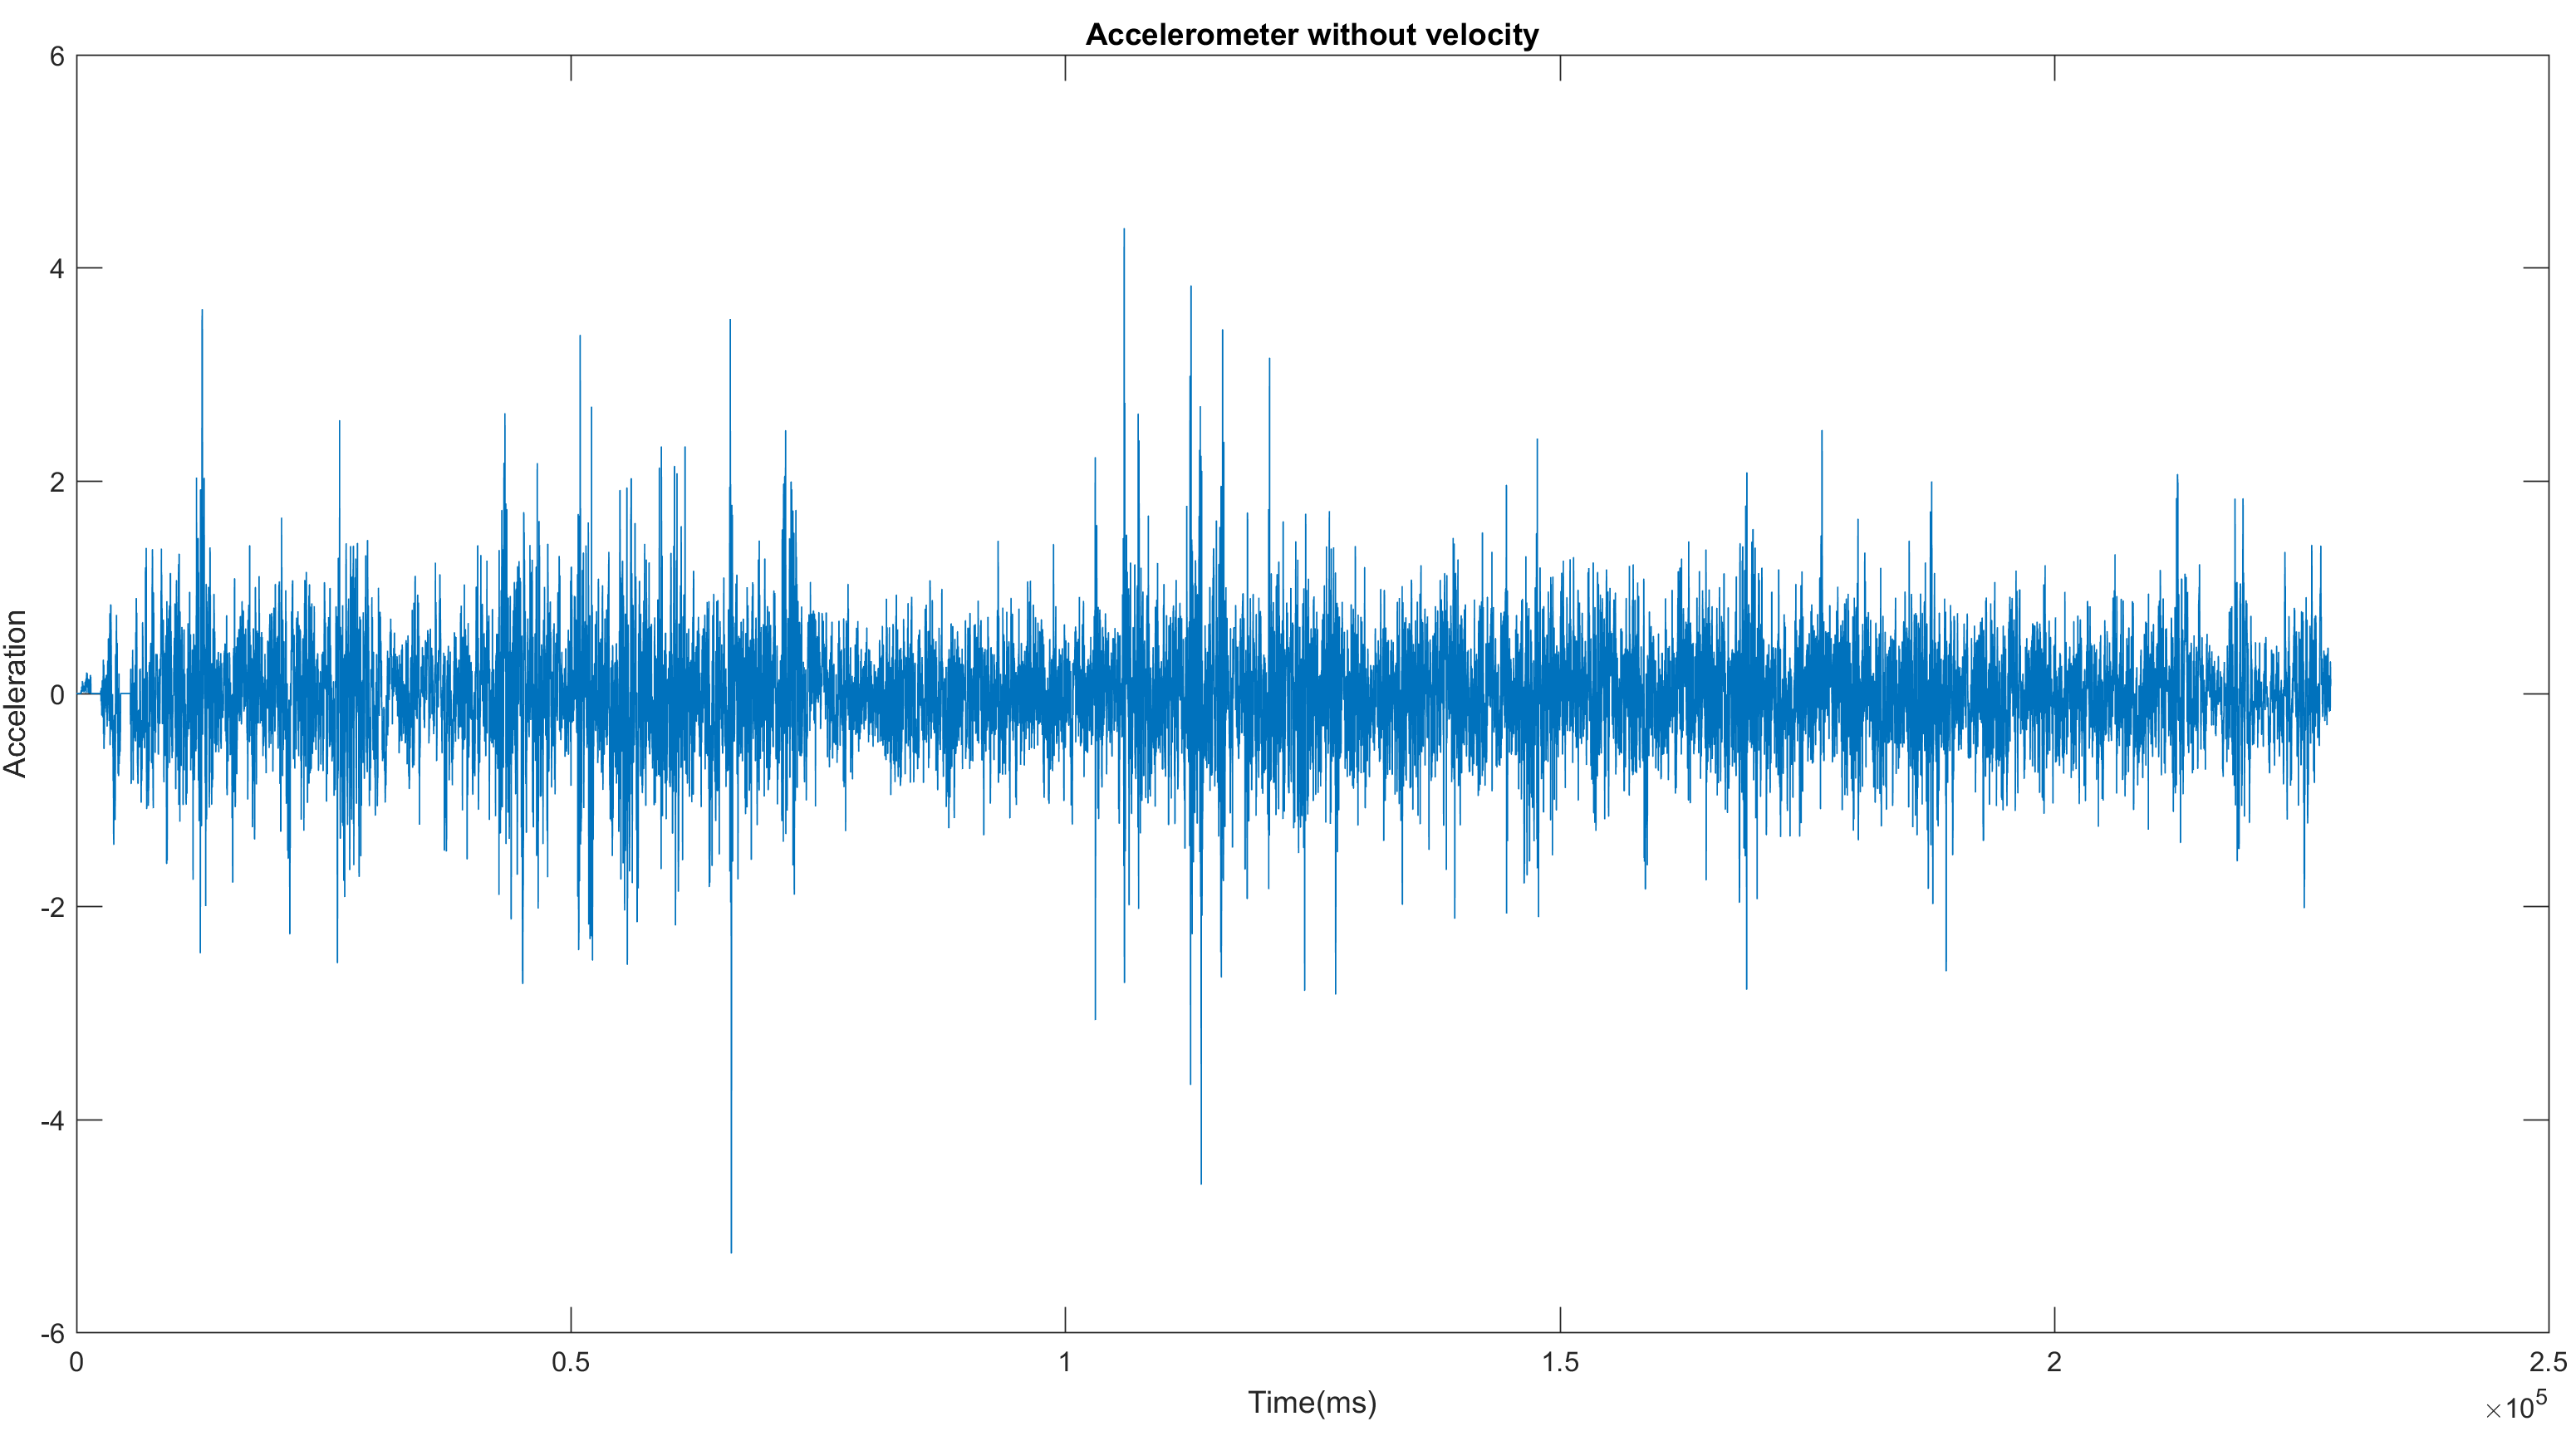
\includegraphics[scale=0.1]{SPANoVelocity}
\end{figure}
\item[4. Remove Engine Vibrations Filter:]After applying the filter, this is also applied, in which the noise components generated by the engine will be smoothed, according to the application seen in the Chapter\ref{ch:Data Analysis} (section:\ref{sc:Data Filtering}, on page:\pageref{sssc:Remove Engine Vibrations Filter})
A figure below show how the filter is applied on the Signal
\begin{figure}[H]
\centering
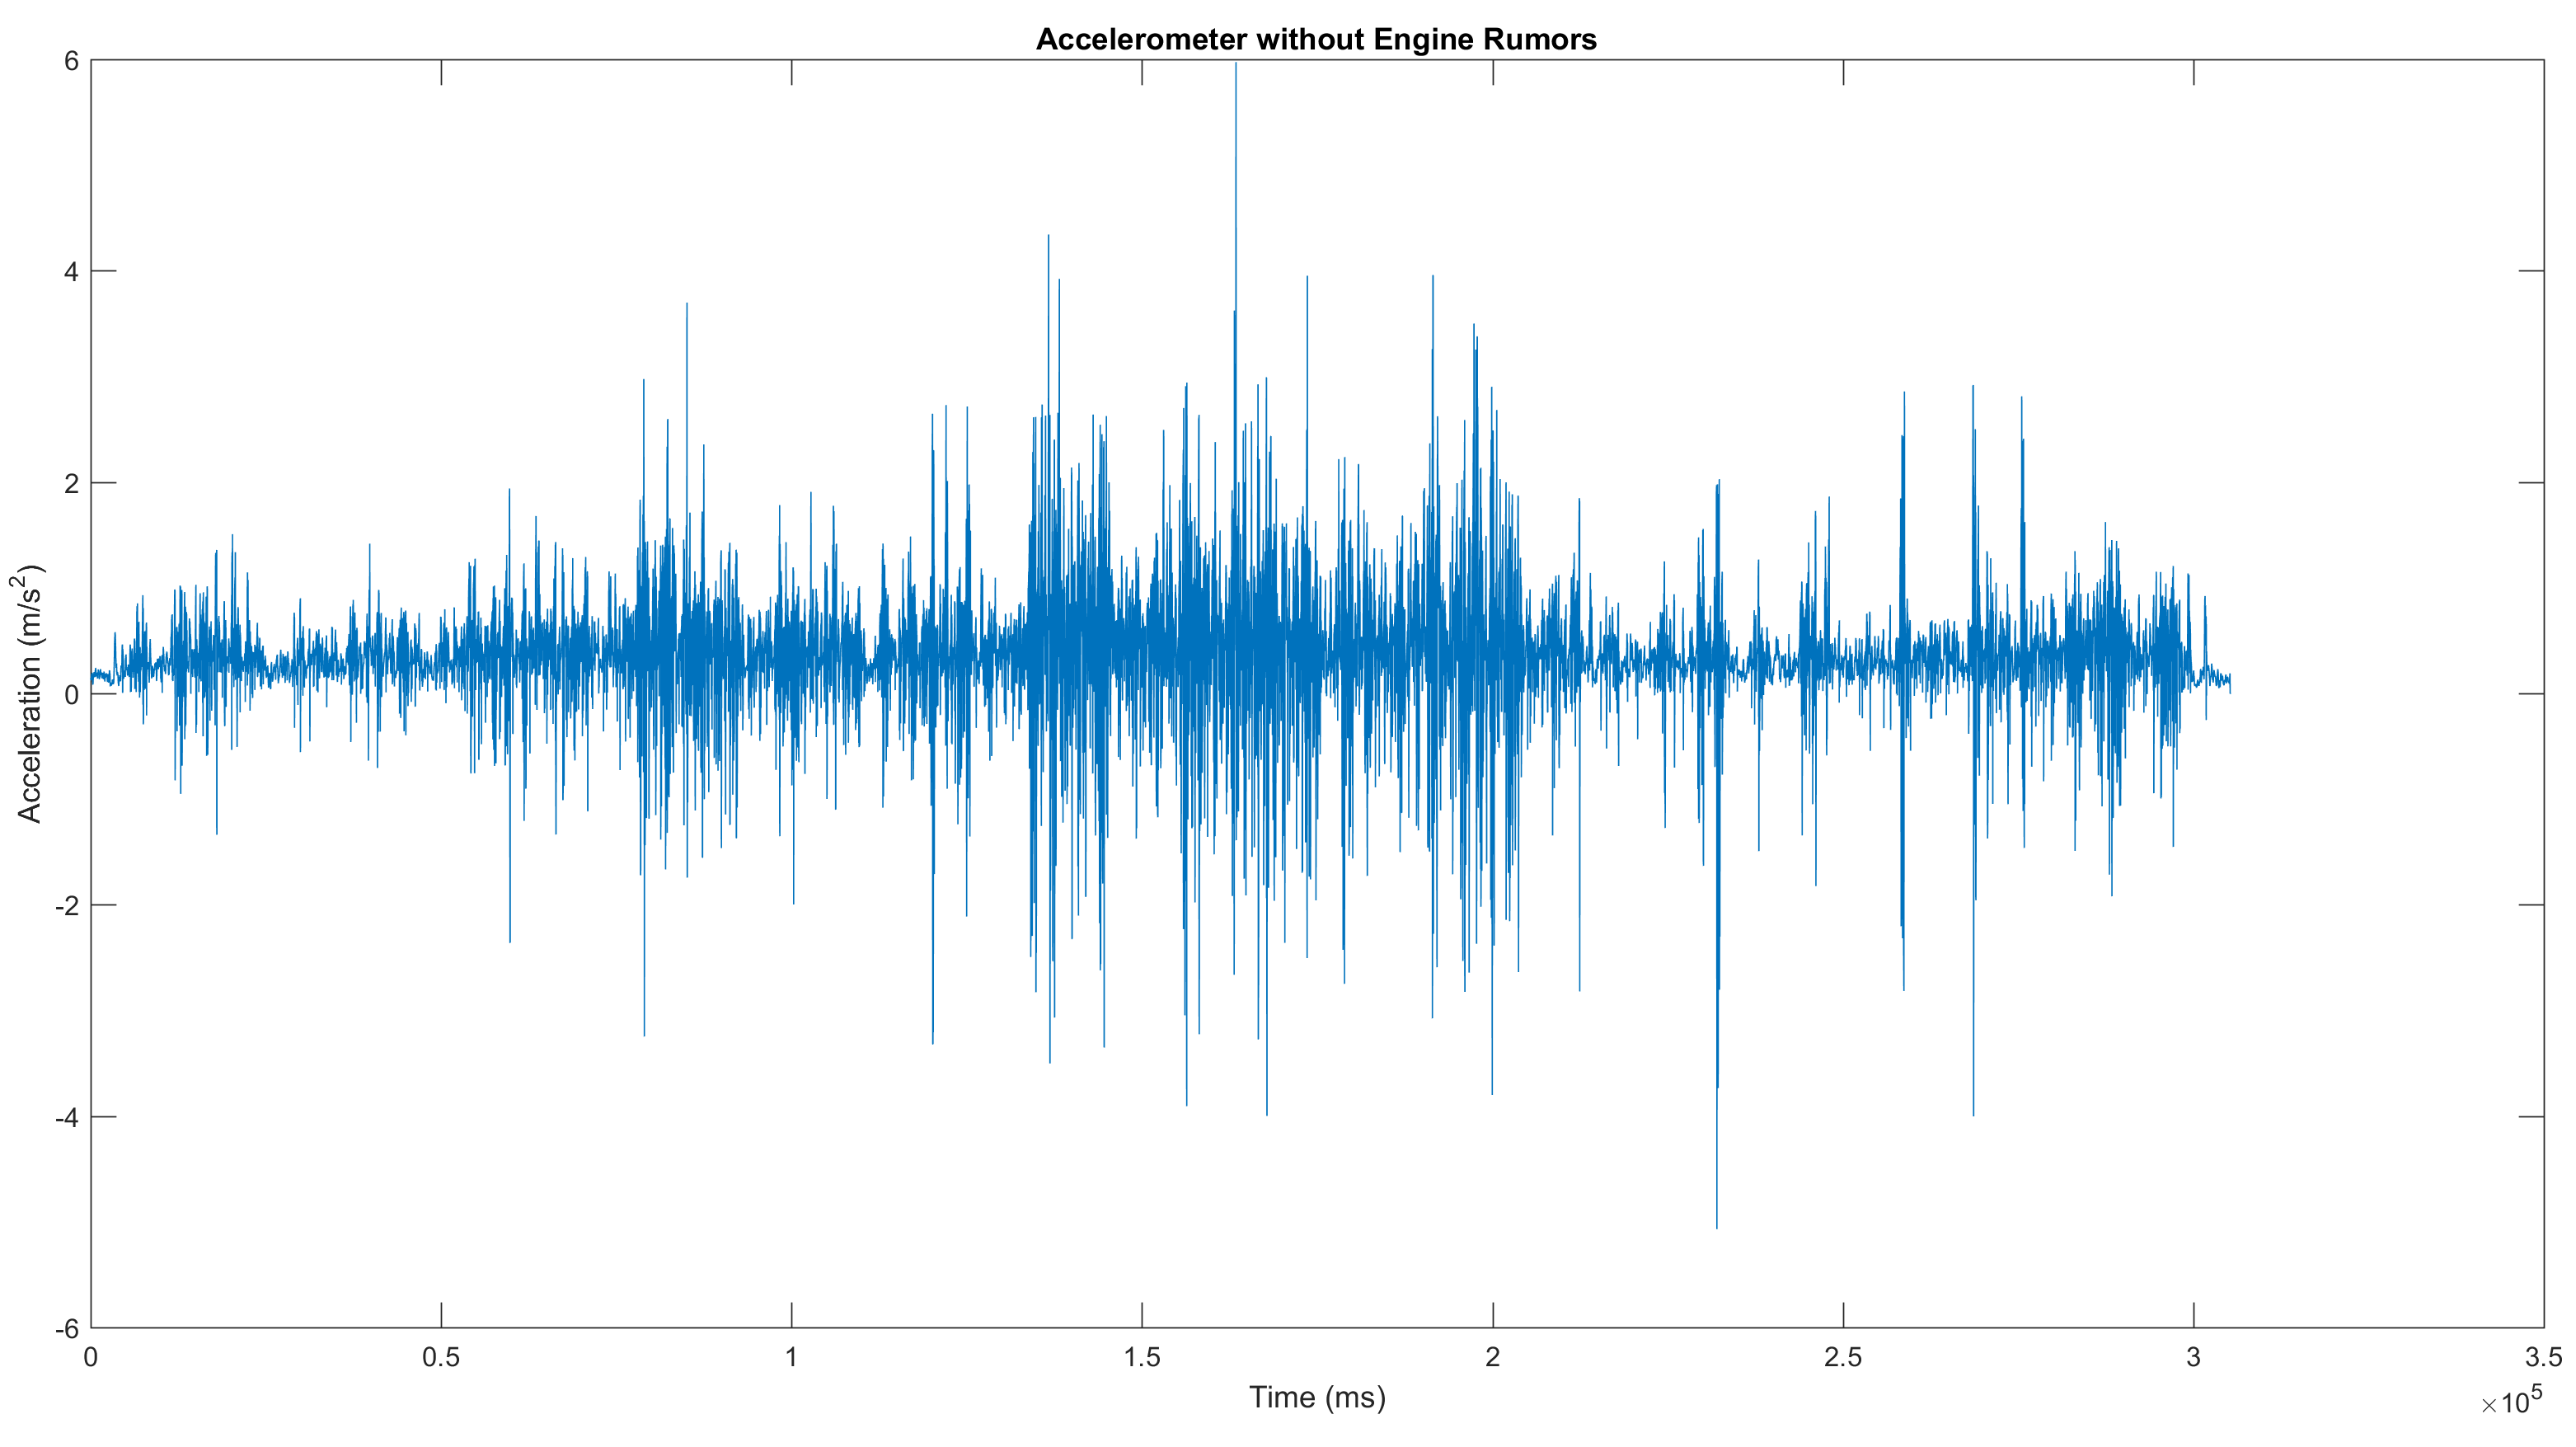
\includegraphics[scale=0.1]{SPANoEngine}
\end{figure}
\item[5. Calculation of the final index:] Ultimately, the final index is calculated. 
This value it is associated with a certain portion of the road ($distance_{segment}$). Following the application of the two previous filters, the Haversine formula will be used (as it is explanained on page: \ref{ssc:Haversine Formula}) to calculate the cumulative GPS distance of points until the $distance_{segment}$ is reached. The new GPS point will be identified by the set of points needed to compose the segment. For the $\chi$ \thinspace \ref{eq:sap} value, it will be calculated by all the acceleration values that are simultaneously read together the GPS points.
A figure below show the result.
\begin{figure}[H]
\centering
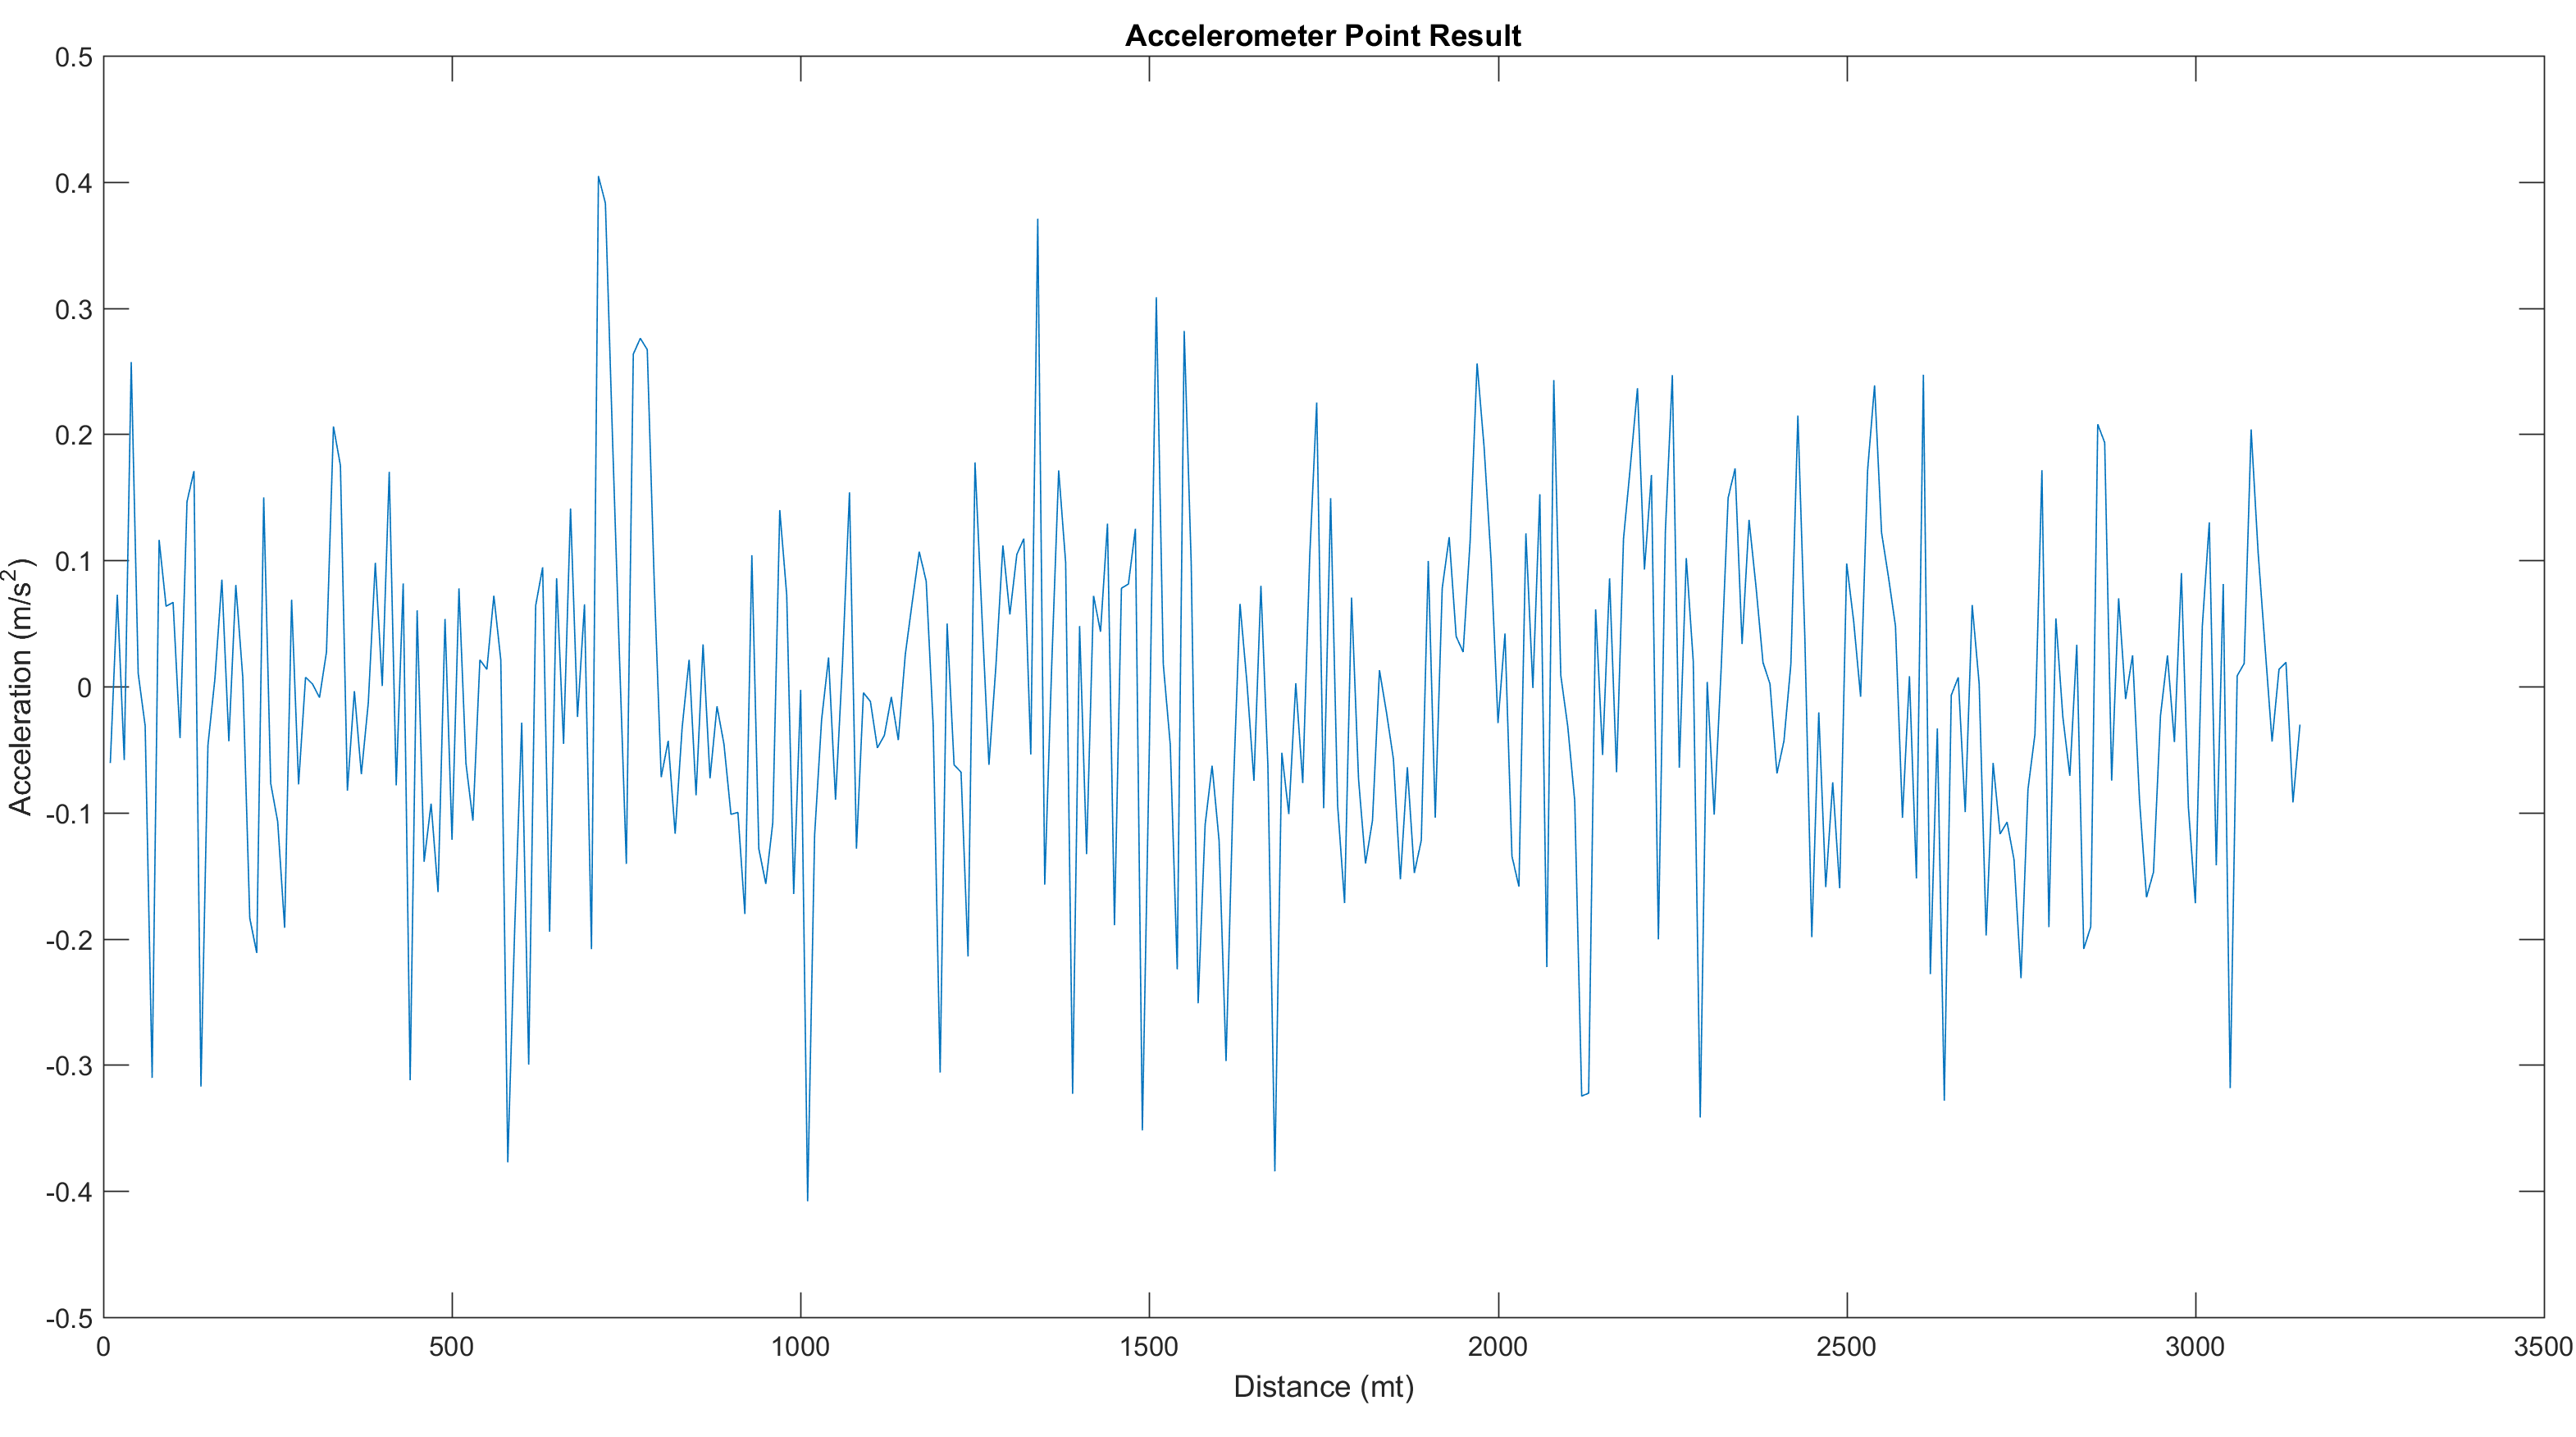
\includegraphics[scale=0.1]{SPAFinal}
\end{figure}
\end{description}
\end{document}